\documentclass[a4paper, 1.5lines]{ctexart}
\usepackage[top=3cm, bottom=2cm]{geometry}
\usepackage{graphicx}
\usepackage{subcaption}
\usepackage{amsmath}
\usepackage{xcolor}
\usepackage{url}
\usepackage{booktabs}
\usepackage{multirow}
%\usepackage{hyperref}
\usepackage[hidelinks]{hyperref} % 加载 hyperref 并隐藏链接边框

%\usepackage[utf8]{inputenc}
%\usepackage[ngerman]{babel} % 加载德语支持

% booktabs 提供 \toprule, \midrule, \bottomrule 等表格命令
\usepackage{booktabs}
% 定义占位命令以避免未定义控制序列错误
\newcommand{\placeholderspace}{}
\usepackage{fancyhdr} % 导入fancyhdr宏包
\usepackage{lipsum}   % 仅用于生成示例文本
\usepackage{float}    % 提供 H 浮动位置选项

% 设置页面样式为fancy
\pagestyle{fancy}
% 自定义页眉内容
\fancyhead[L]{} % 左侧页眉
\fancyhead[C]{\textbf{Physics-experiment Reporting Letter:\\Optical Multi-channel and H-D spectroscopy}} % 中间页眉
\fancyhead[R]{ } % 右侧页眉
% 自定义页脚内容
\fancyfoot[L]{ } % 左侧页脚
\fancyfoot[C]{\thepage} % 中间页脚显示页码
\fancyfoot[R]{ } % 右侧页脚
% 改变页眉线的粗细
\renewcommand{\headrulewidth}{1.4pt}
% 改变页脚线的粗细
\renewcommand{\footrulewidth}{0.pt}





\title{氦氖激光的纵横模分析和模分裂}
\author{实验人：唐亿\qquad 学号：202311998381\qquad 指导教师：弓文平}
\date{实验日期：2025.11.21}


\begin{document}
    
    \maketitle
    
    \begin{abstract}
         该报告探讨了氦氖（He-Ne）激光器的模谱特性，包括纵模和横模的测量，以及纵模分裂和模竞争的现象。通过使用共焦球面扫描干涉仪，实验成功地测量了短管和长管的模谱分布、激光器的出光带宽，并通过改变石英晶体的角度实现了纵模分裂的观察。
        
         \textbf{\textbf{关键词：激光\quad 横模\quad 纵模\quad 出光带宽\quad 模分裂}}
    \end{abstract}
    
    \section{引言}
        激光器的物理机理与性能评估是现代光学技术中的核心内容，而对其模结构的测量与分析则是理解这些问题的关键步骤。在诸多气体激光器中，氦氖激光器因输出稳定、操作简便、结构成熟而被广泛用于实验教学和工程应用。本实验围绕氦氖激光器的频谱特性展开，通过对其输出光的模谱进行测量，观察不同振荡模式在腔内形成的规律，进而讨论纵模和横模在频域与空间分布上的特点。此外，激光谐振腔内的双折射效应会改变模式间的频率关系，从而引起纵模分裂。本实验也将通过对测得的模谱进行分析，验证这一现象并加深对氦氖激光器工作机制的理解。
    \section{原理}
        \subsection{激光的产生}
            \subsubsection{受激辐射与粒子数反转}
            Einstein在1916年唯象的提出当光与原子相互作用时，可以有自发辐射、受激辐射和吸收。受激辐射与自发辐射的最本质区别是受激辐射的光宇入射光的频率、相位、偏振状态和传播方向都完全相同，相较于自发辐射的光，具有更好的相干性。

            粒子数反转就是在受激辐射和吸收的过程中发生的。当频率为$\nu$的光照射到具有能级$E_2,E_1(E_2-E_1 = h\nu)$的介质时，受激辐射会加强入射光，而吸收会减弱。
            设两能级上的粒子数密度分别为$N_1,N_2$，入射光的单色辐射能量密度为$\rho_v$，则有

            \centerline{$\mathrm{d}N_{21} = B_{21} N_2 \rho_v \mathrm{d}t$}

            \centerline{$\mathrm{d}N_{12} = B_{12} N_1 \rho_v \mathrm{d}t$}

            其中$\mathrm{d}N_{21}$为受激辐射的光子数，$\mathrm{d}N_{12}$为吸收的光子数。
            对于一个特定的辐射过程，只有当受激发射的速率 ($\mathrm{d}N_{21}$) 超过受激吸收的速率 ($\mathrm{d}N_{12}$) 时，即满足 $\mathrm{d}N_{21} > \mathrm{d}N_{12}$，入射光才能在介质中获得增益。
            然而，在通常的热平衡状态下，能级粒子数比值的玻尔兹曼分布决定了
            $$
            \frac{\mathrm{d}N_{21}}{\mathrm{d}N_{12}} = \frac{g_1 N_2}{g_2 N_1} = \mathrm{e}^{-(E_2 - E_1)/kT} < 1
            $$
            这使得该介质对光线表现出固有的损耗特性。
            因此，若要实现对光的净增益，必须通过外部手段精确调控，以创造 $\frac{\mathrm{d}N_{21}}{\mathrm{d}N_{12}}>1$ 的非平衡条件。
            这种被刻意达成的非平衡分布状态，在物理学中被称为“粒子数反转”。
            \subsubsection{介质增益损耗的唯象描述}
            介质对光波的放大能力由{增益系数} $G$ 来量化，其定义为光强 $I$ 通过单位长度 $\mathrm{d}z$ 介质后的相对增长率：
            $$
            G = \frac{\mathrm{d}I(z)}{I(z)\mathrm{d}z}
            $$
            若考虑一个简化的二能级系统，其频率相关的增益系数 $G(\nu)$ 可以表示为：
            $$
            G(\nu) = \left(N_2 - N_1\frac{g_2}{g_1}\right) \frac{n}{c}B_{21}h\nu g(\nu)
            $$
            其中，$n$ 代表介质的折射率，$c$ 为真空中的光速，$g(\nu)$ 是描述谱线展宽的线型函数。需要注意的是，光在介质中传播时不可避免地会伴随固有损耗 $\alpha$。

            当光在谐振腔内反复振荡时，仅有那些{净增益超过损耗}（即往返一次后增益大于损耗）的特定频率光波能够得到持续增强，最终在腔内建立起稳定的光场分布，并实现激光输出。激光器开始工作的{阈值条件}是增益必须克服全部损耗，即 $G(\nu) \ge \alpha$。我们将满足 $G(\nu) = \alpha$ 时的增益系数定义为{阈值增益系数} $G_{\text{阈}}$。所有使得 $G(\nu) > G_{\text{阈}}$ 的频率区间，即为激光器实际的{出光带宽}。
        \subsection{激光模式}
            \subsubsection{纵模}
            在谐振腔内，只有沿腔轴方向传播的光波，其往返一周的总光程为波长 $\lambda$ 的整数倍时，才能形成稳定的驻波场分布。这一条件构成了腔内振荡模式的基础，即：
            $$
            2L\mu = q\lambda
            $$
            其中 $L$ 是腔长，$\mu$ 是介质的折射率（对于 He-Ne 激光器，$\mu \approx 1$），而 $q$ 是一个\textbf{大的整数}，被称为纵模序号。

            基于此驻波条件，可以推导出谐振腔允许的激光振荡频率 $v_q$ 必须满足：
            $$
            v_q = q \cdot \frac{c}{2\mu L}
            \quad \text{或} \quad
            v_q = q \cdot \frac{c}{2L} \quad (\text{当 } \mu \approx 1 \text{ 时})
            $$
            这表明，稳定光场分布的频率是 $\frac{c}{2\mu L}$ 的整数倍。满足这一条件的稳定驻波场被称为\textbf{纵模}。相邻纵模之间的频率间隔 $\Delta v_q$ 是恒定的，其大小可由下式确定：
            $$
            \Delta v_q = \frac{c}{2\mu L}
            $$
            
            \subsubsection{横模}
            光波在谐振腔内传播时，不仅沿轴向形成纵模驻波，由于光束的截面和腔镜的限制，在垂直于传播方向上也存在不同的场分布，这些分布被称为\textbf{横模}。每个横模分布由两个模序数 $m$ 和 $n$ 标记，通常写作 $\text{TEM}_{mn}$。其中，$\text{TEM}_{00}$ 模是最低阶的横模，其光强沿轴向对称分布，是理想的激光模式。当 $m$ 和 $n$ 不为零时，光束的横截面会出现暗区和光斑的分裂。

            实验中测量的横模序数 $m$ 和 $n$ 指示了光斑在 $x$ 轴和 $y$ 轴方向上的节点数。不同横模之间的频率间隔 $\Delta v_{\text{横}}$ 由纵模序号 $q$ 和横模序号 $m, n$ 共同决定：
            $$
            \Delta v_{\text{横}} = v_{m,n,q} - v_{m',n',q'}
            $$
            横模的频率间隔 $\Delta v_{\text{横}}$ 通常远小于相邻纵模的频率间隔 $\Delta v_q$，即 $\Delta v_q \gg \Delta v_{\text{横}}$。

            根据不同的谐振腔类型，其横模频率间隔 $\Delta v_{\text{横}}$ 的计算公式也不同，例如：

            \begin{enumerate}
                \item \textbf{平面平行镜腔} ($\text{TEM}_{m,n,q}$ 与 $\text{TEM}_{m',n',q}$ 之间)：
                $$
                \Delta v_{\text{横}} = \frac{c}{2\mu L} \frac{1}{\pi} \left(2\Delta m + \Delta m^2 + 2\Delta n + \Delta n^2\right)^{\frac{1}{2}}
                $$
                其中，$N = \frac{\mu a^2}{L\lambda}$ 为菲涅耳数，$a$ 为激光孔径半径。
    
                \item \textbf{共焦腔}（$R_1=R_2=L$）：其横模间隔 $\Delta v_{\text{横}}$ 是相邻纵模间隔 $\Delta v_q$ 的一半：
                $$
                \Delta v_{\text{横}} = \frac{c}{4\mu L} (\Delta m + \Delta n)
                $$
    
                \item \textbf{非共焦的通用稳定腔}：
                $$
                \Delta v_{\text{横}} = \frac{c}{2\mu L} \left(\frac{1}{\pi} (\Delta m + \Delta n) \arccos\left[\left(1-\frac{L}{R_1}\right)\left(1-\frac{L}{R_2}\right)\right]^{\frac{1}{2}}\right)
                $$
                其中 $R_1$ 和 $R_2$ 为两个反射镜的曲率半径。
            \end{enumerate}
    \section{实验}
        本次实验旨在对氦氖（He-Ne）激光器的工作特性进行深入分析。核心内容包括两方面：激光模谱的测量与分析，以及腔内元件对模式的影响研究。具体操作中，我们首先利用扫描干涉仪精确测量了不同腔长 He-Ne 激光管（短管和长管）的纵模频率间隔 ($\Delta v_q$)，同时结合横向光场分布对长管的横模成分进行了识别和量化。其次，在纵模分裂和模竞争实验中，我们利用激光频率分裂专用激光器，通过调节腔内石英晶片的晶轴角度，引入双折射效应，从而实现纵模的频率分裂；最终通过偏振片分析了分裂后两条谱线的偏振特性，以探究双折射元件对腔内模式的调控作用。

\subsection{实验仪器原理}

\subsubsection{He-Ne 激光器原理}
He-Ne 激光器的核心是一个包含增益介质和光学谐振腔的系统。谐振腔由两个相对设置的介质膜反射镜构成，腔内填充 He 和 Ne 混合气体作为工作物质。实现激光增益的前提是粒子数反转：即通过放电激励等泵浦手段，使高能级 $E_2$ 上的粒子数多于低能级 $E_1$ 上的粒子数。当光束通过此介质时，频率 $\nu = (E_2 - E_1)/h$ 的光被放大，即产生了增益。由于自然、碰撞和多普勒效应等因素，能级具有一定的宽度，导致增益系数 $G(\nu)$ 随频率 $\nu$ 变化，其分布曲线（增益曲线）与谱线线型函数 $g(\nu)$ 具有相同的形状。

\subsubsection{石英晶体对激光模式的影响}

\paragraph{双折射效应}
石英晶体作为一种天然的双折射材料，使通过它的光束分裂成寻常光（o光）和非寻常光（e光）。由此产生的两束光的折射率分别为 $n'$ 和 $n''$，导致两者间存在光程差 $\delta$，表达式如下：
$$
\delta = ( n'' - n' )h
$$
其中 $h$ 是晶片厚度，$n'$ 和 $n''$ 分别是 o 光和 e 光的折射率，$n_o$ 和 $n_e$ 是主折射率，而 $n''$ 由晶轴与光线夹角 $\theta$ 决定：
$$
n'' = \left(\dfrac{\sin^2\theta}{n_e^2} + \dfrac{\cos^2\theta}{n_o^2}\right)^{-1/2}
$$
因此，通过改变晶轴与光线的夹角 $\theta$，可以精确控制 o 光和 e 光之间的光程差 $\delta$。

\paragraph{模式分裂}
将具有双折射特性的元件置入激光谐振腔内，相当于为 o 光和 e 光分别设置了不同的等效腔长 $L$。原本单一的谐振腔长因此“分裂”为两个，导致腔内谐振频率发生分裂。根据驻波条件导出的频率与腔长的关系 $\nu = \frac{c}{2L} q$，引入的光程差 $\delta$ 可视为腔长变化 $\Delta L$。由此导致的频率分裂量 $|\Delta \nu|$ 与光程差 $\delta$ 之间的关系为：
$$
|\Delta \nu| = \frac{\nu}{L} \delta
$$
本实验正是通过旋转腔内石英晶片以改变 $\delta$，实现对纵模频率的人工分裂。通过放置偏振片，可以观察和确定分裂出的两条谱线光的偏振方向。

\subsubsection{共焦球面扫描干涉仪}

共焦球面扫描干涉仪由两个曲率半径 $R$ 相等、距离 $L$ 也等于 $R$ 的球面高反镜组成，构成了共焦系统。其独特的几何结构确保了入射光在腔内经四次反射后与入射光重合，总光程差 $\Delta \approx 4L$。满足相长干涉的频率 $\nu$ 为：
$$
\nu = \frac{c}{\lambda} = \frac{K c}{4 L}
$$
干涉仪通过压电陶瓷环驱动一面镜子，使腔长 $L$ 在 $L_0$ 附近微小周期性变化 $\delta L$。在 $\delta L$ 远小于 $L_0$ 的一阶近似下，频率变化量 $\Delta \nu$ 与 $\delta L$ 成正比，进而与施加在压电陶瓷上的电压呈线性关系：
$$
\Delta \nu \propto \delta L \propto V
$$
因此，示波器的横坐标（电压）与干涉仪的频率变化同步，实现了频率扫描。频率间隔 $\Delta \nu$ 可通过示波器读数 $\Delta x$ 和干涉仪的自由光谱区（Free Spectral Range, FSR）$\Delta \nu_{FSR}$（已知的基准频率间隔）进行换算：
$$
\dfrac{\Delta \nu}{\Delta x} = \dfrac{\Delta \nu_{FSR}}{\Delta x_{FSR}}
$$
其中，FSR $\Delta \nu_{FSR} = \frac{c}{4 L}$ 决定了干涉仪能够有效测量的最大不重叠频率范围。本实验所用干涉仪的 FSR 为 $1875 \mathrm{MHz}$。

\subsection{实验方法}
\begin{enumerate}
    \item \textbf{仪器调节与模谱观测}
    首先，对激光器与扫描干涉仪进行同轴粗调，使激光束射入干涉仪光栏孔。运行程序输出锯齿波，精细调节干涉仪的方位，使入射光与反射光重合，并使输出光斑对准光电二极管接收面。通过微调干涉仪，观察示波器上的模谱信号，目标是使信号的峰峰值达到最大，从而确保最佳耦合。
    
    \item \textbf{激光偏振态与模分裂分析}
    在激光纵模分裂实验中，首先调整腔内石英晶片的晶轴角度，以产生足够明显的纵模分裂间距。随后，在激光输出端与扫描干涉仪之间放置偏振片 P。通过旋转偏振片 P，观察示波器上两个分裂谱线幅值的变化，进而实验性地确定分裂后两谐振频率光波的偏振关系。
\end{enumerate}
            
    \section{结果与分析讨论}
        \subsection{两根氦氖激光管的模谱分布的测量}

在扫描干涉仪的示波器上，那些满足增益大于损耗条件的激光模式以尖峰的形式呈现，尖峰间的相对位置精确反映了各模式的频率关系。在进行读数时，需要根据自由光谱区（FSR）的范围来准确区分相邻纵模和跨 FSR 的模式。

\paragraph{短管模谱分布}
对于短激光管的模谱，在一个 FSR 内仅观察到两个强度峰（如图\ref{fig:short}所示）。根据纵模间隔的定义，我们将同一 FSR 内间距最小的两个峰值视为相邻纵模的频率峰。例如，图\ref{fig:short}中峰 1 、 2 和 3 构成一组相邻纵模，峰 4、5 和 6 构成另一组，而峰 1 和 4 之间则代表一个完整的自由光谱区。

\paragraph{长管模谱分布}
相比短管，长激光管的模谱分布更为复杂，其中包含了横模成分（如图\ref{fig:long}和\ref{fig:llong}所示）。图\ref{fig:llong}中标记的 \textbf{I}、\textbf{II} 区域分别对应于不同的自由光谱区。在长管的模式结构中，我们识别出相邻纵模（分别为峰 1、2/3/4），以及两组相邻横模（分别为峰 2/3），且3、4之间有一个横模被淹没。同时峰 1 的相邻横模信号已不可见。

\begin{figure}[h!]
    \centering
    \begin{subfigure}{0.47\textwidth}
        \centering
        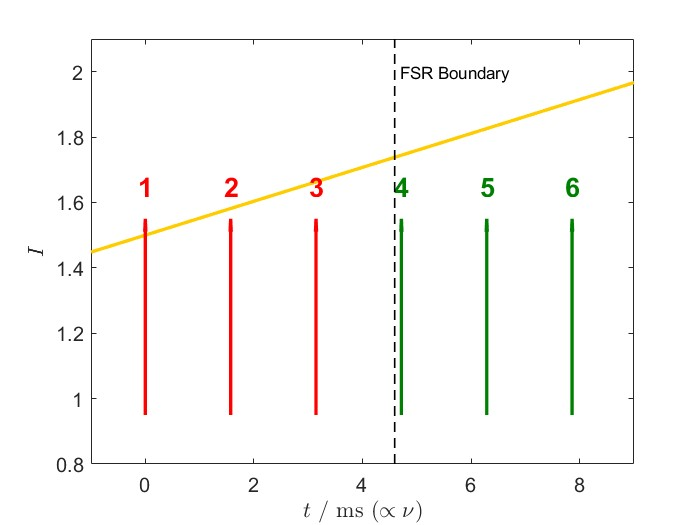
\includegraphics[width=\textwidth]{fig//short} % 假设图文件已上传
        \captionsetup{font=small}
        \caption{短管的模谱分布示意图}
        \label{fig:short}
    \end{subfigure}
    \hfill
    \begin{subfigure}{0.47\textwidth}
        \centering
        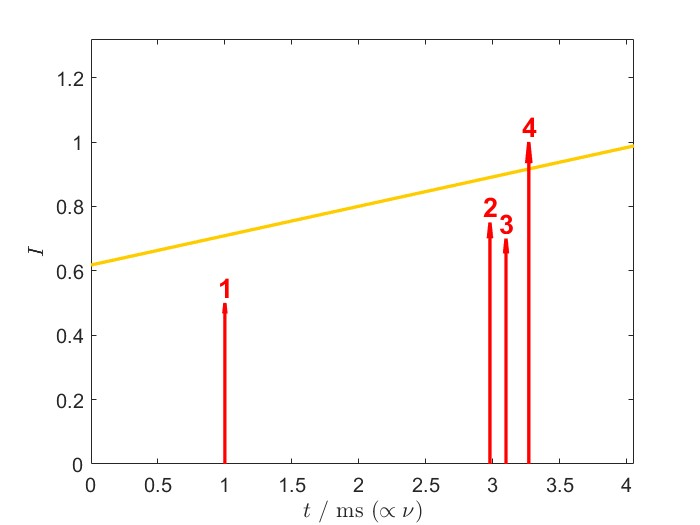
\includegraphics[width=\textwidth]{fig//long_2} % 假设图文件已上传
        \captionsetup{font=small}
        \caption{长管同一自由光谱区的横模、纵模分布示意图}
        \label{fig:long}
    \end{subfigure}
    \hfill
    \begin{subfigure}{\textwidth}
        \centering
        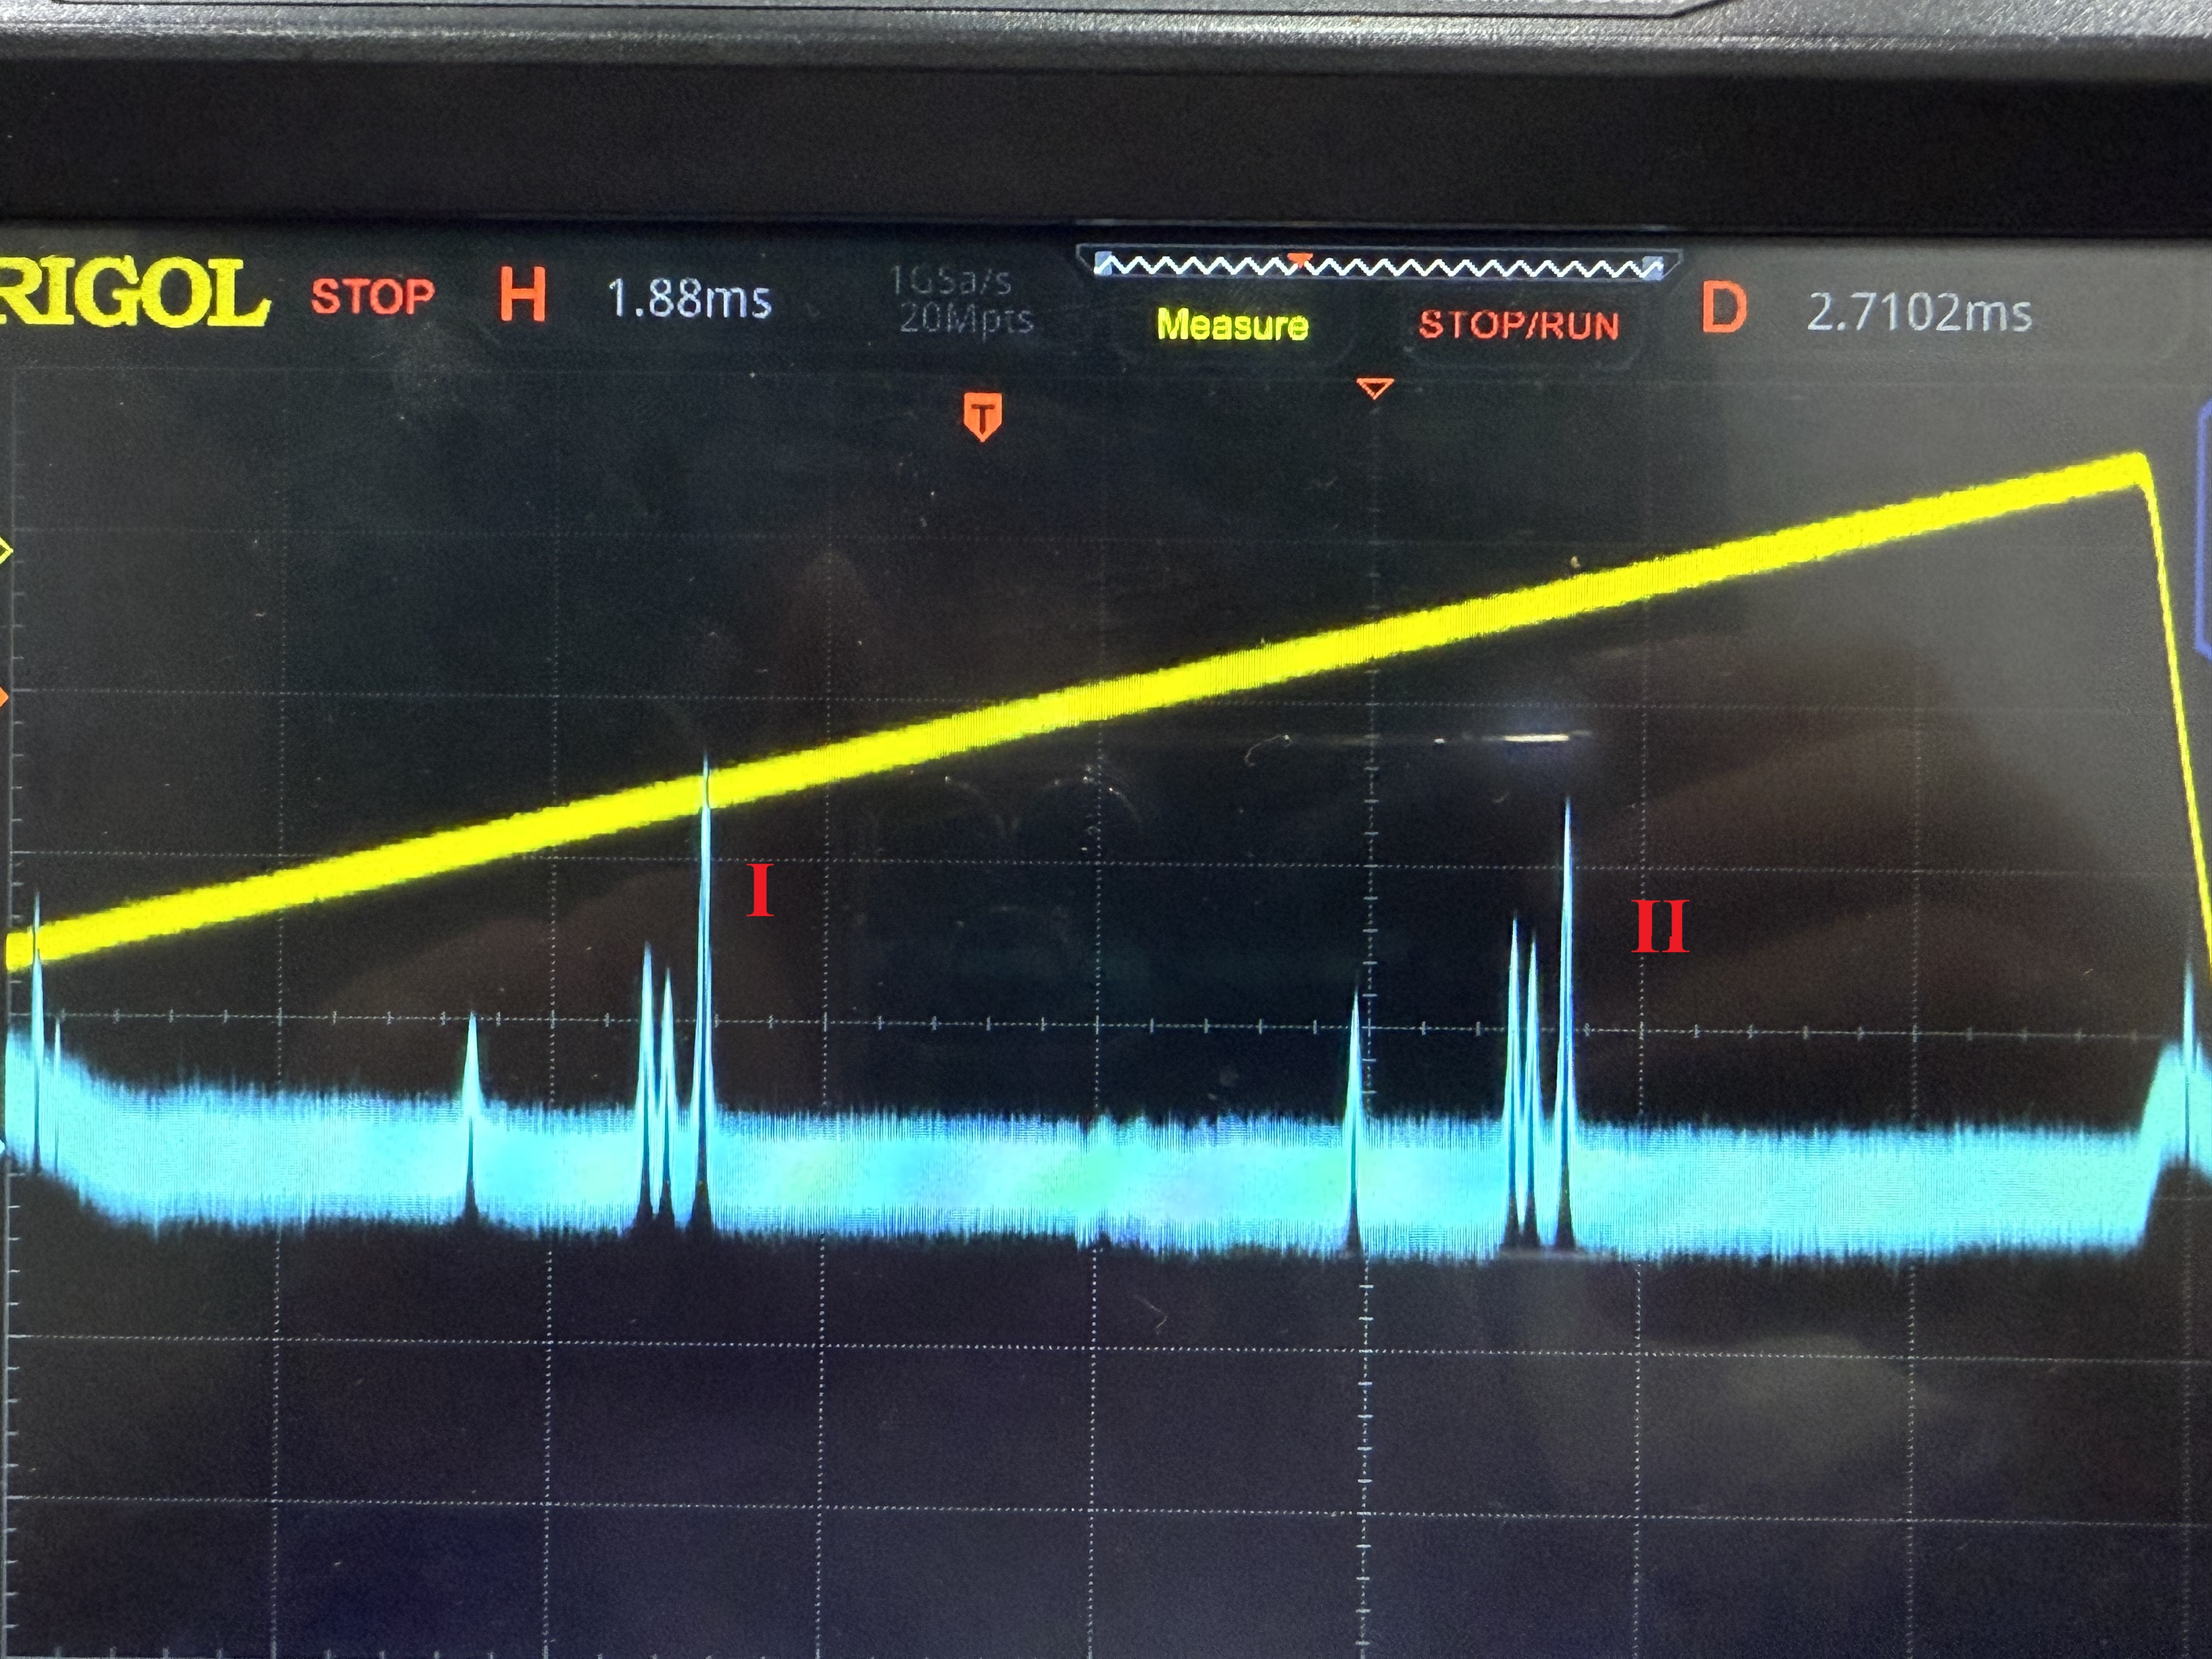
\includegraphics[width=0.7\textwidth]{fig//long_1} % 假设图文件已上传
        \captionsetup{font=small}
        \caption{长管的模谱分布（\textbf{I}、\textbf{II}区域为不同的自由光谱区）}
        \label{fig:llong}
    \end{subfigure}
    \caption{两根氦氖激光管的模谱分布的示波器测量图}
    \label{fig:tube}
\end{figure}


\subsubsection{理论与实验数据对比}

实验中使用的激光管信息如下：短管长度 $L_{\text{短}} = 238 \mathrm{mm}$，长管长度待测，反射镜曲率半径$R = 100 \mathrm{cm}$。
\begin{itemize}
    \item 短管纵模间隔 $\Delta \nu_{\text{短}, \text{理论}} = 630.25 \mathrm{MHz}$
\end{itemize}

\subsubsection{短管纵模间隔的测定}

短管模谱的数据记录（示波器横坐标 $x$）如表 1 所示。

\begin{table}[h!]
    \centering
    \caption{短管模谱的示波器读数}
    \begin{tabular}{ccccccc}
        \toprule
        峰编号 & 1 & 2 & 3 & 4 & 5 & 6 \\
        \midrule
        $x$/ms & -2.488 & -0.903 & 0.629 & 2.254 & 3.781 & 5.382 \\
        \bottomrule
    \end{tabular}        
    \label{tab:short_data}
\end{table}

经计算，自由光谱区的平均间隔 $\Delta x_{FSR} = 4.593 \mathrm{ms}$，相邻纵模的平均间隔 $\Delta x_{\text{纵}} = 1.572 \mathrm{ms}$。根据干涉仪的 FSR $\Delta \nu_{FSR} = 1875 \mathrm{MHz}$，换算得到的实验频率间隔为：
$$
\Delta \nu_{\text{实验}} = \dfrac{\Delta \nu_{FSR}}{\Delta x_{FSR}}\ \Delta x_{\text{纵}} = 641.74 \mathrm{MHz}
$$


\subsubsection{长管纵模与横模间隔的测定}

长管模谱在两个 FSR 区域 $\mathbf{I}$、$\mathbf{II}$ 的数据记录如表 2 所示。

\begin{table}[h!]
    \centering
    \caption{长管模谱的示波器读数}
    \begin{tabular}{cccccccc}
        \toprule
        峰编号 & 1 & 2 & 3 & 4  \\
        \midrule
        $x_\mathbf{I}$/ms & -3.478 & -2.274 & -2.143 & -1.898  \\
        $x_\mathbf{II}$/ms & 2.613 & 3.703 & 3.835 & 4.060  \\
        \bottomrule
    \end{tabular}
    \label{tab:long_data}
\end{table}

经计算，自由光谱区的平均间隔 $\Delta x_{FSR} =  5.971\mathrm{ms}$。

\paragraph{相邻纵模间隔}
相邻纵模的平均间隔 $\Delta x_{\text{纵}} = 1.514 \mathrm{ms}$。换算得到的实验频率间隔为：
$$
\Delta \nu_{\text{纵}, \text{实验}} = \dfrac{\Delta \nu_{FSR}}{\Delta x_{FSR}}\ \Delta x_{\text{纵}} = 475.42 \mathrm{MHz}
$$
可反解得
$$
L = \dfrac{c}{2 \Delta \nu_{\text{纵}, \text{实验}}} = 315.1 \mathrm{mm}
$$

\paragraph{相邻横模间隔}
相邻横模的平均间隔 $\Delta x_{\text{横}} = 0.125 \mathrm{ms}$。换算得到的实验频率间隔为：
$$
\Delta \nu_{\text{横}, \text{实验}} = \dfrac{\Delta \nu_{SR}}{\Delta x_{SR}}\ \Delta x_{\text{横}} = 39.25 \mathrm{MHz}
$$


\paragraph{横向模成分分析}
结合对长管出射光束横向光场分布的观测（如图\ref{fenbu}所示），由于光场内部分割为六块亮区，可以推断出长管的横模成分可能包含 $\mathrm{TEM}_{0,0}$、$\mathrm{TEM}_{0,1} $、$\mathrm{TEM}_{1,0}$ 、 $\mathrm{TEM}_{1,1} $ 、$\mathrm{TEM}_{2,0} $ 、$\mathrm{TEM}_{2,1} $ 六种模式。

\begin{figure}
    \centering
    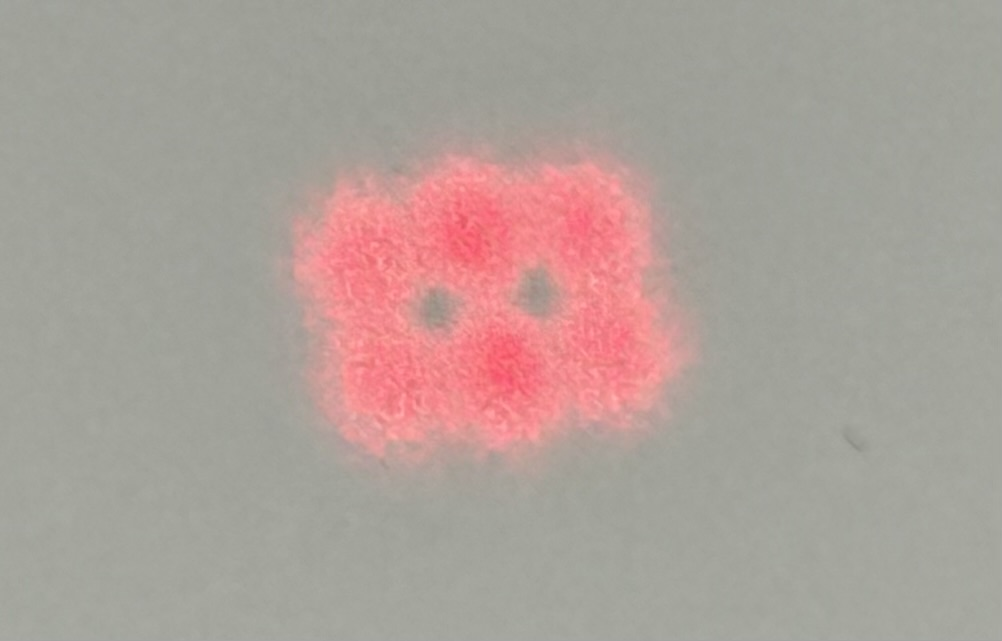
\includegraphics[width=0.4\textwidth]{fig//fenbu} % 假设图文件已上传
    \captionsetup{font=small}
    \caption{长管出射光束的横向光场分布示意图}
    \label{fenbu}
\end{figure}

\subsection{观测氦氖激光器的纵模分裂和模竞争}

实验除了测量激光管的模谱分布外，还测定了氦氖激光器的出光带宽，并进一步探究了石英晶体双折射效应导致的纵模分裂现象及其模式偏振关系。

\begin{figure}[h!]
    \centering
    \begin{subfigure}{0.47\textwidth}
        \centering
        % 请将图文件 band.png 放置在 fig 目录下
        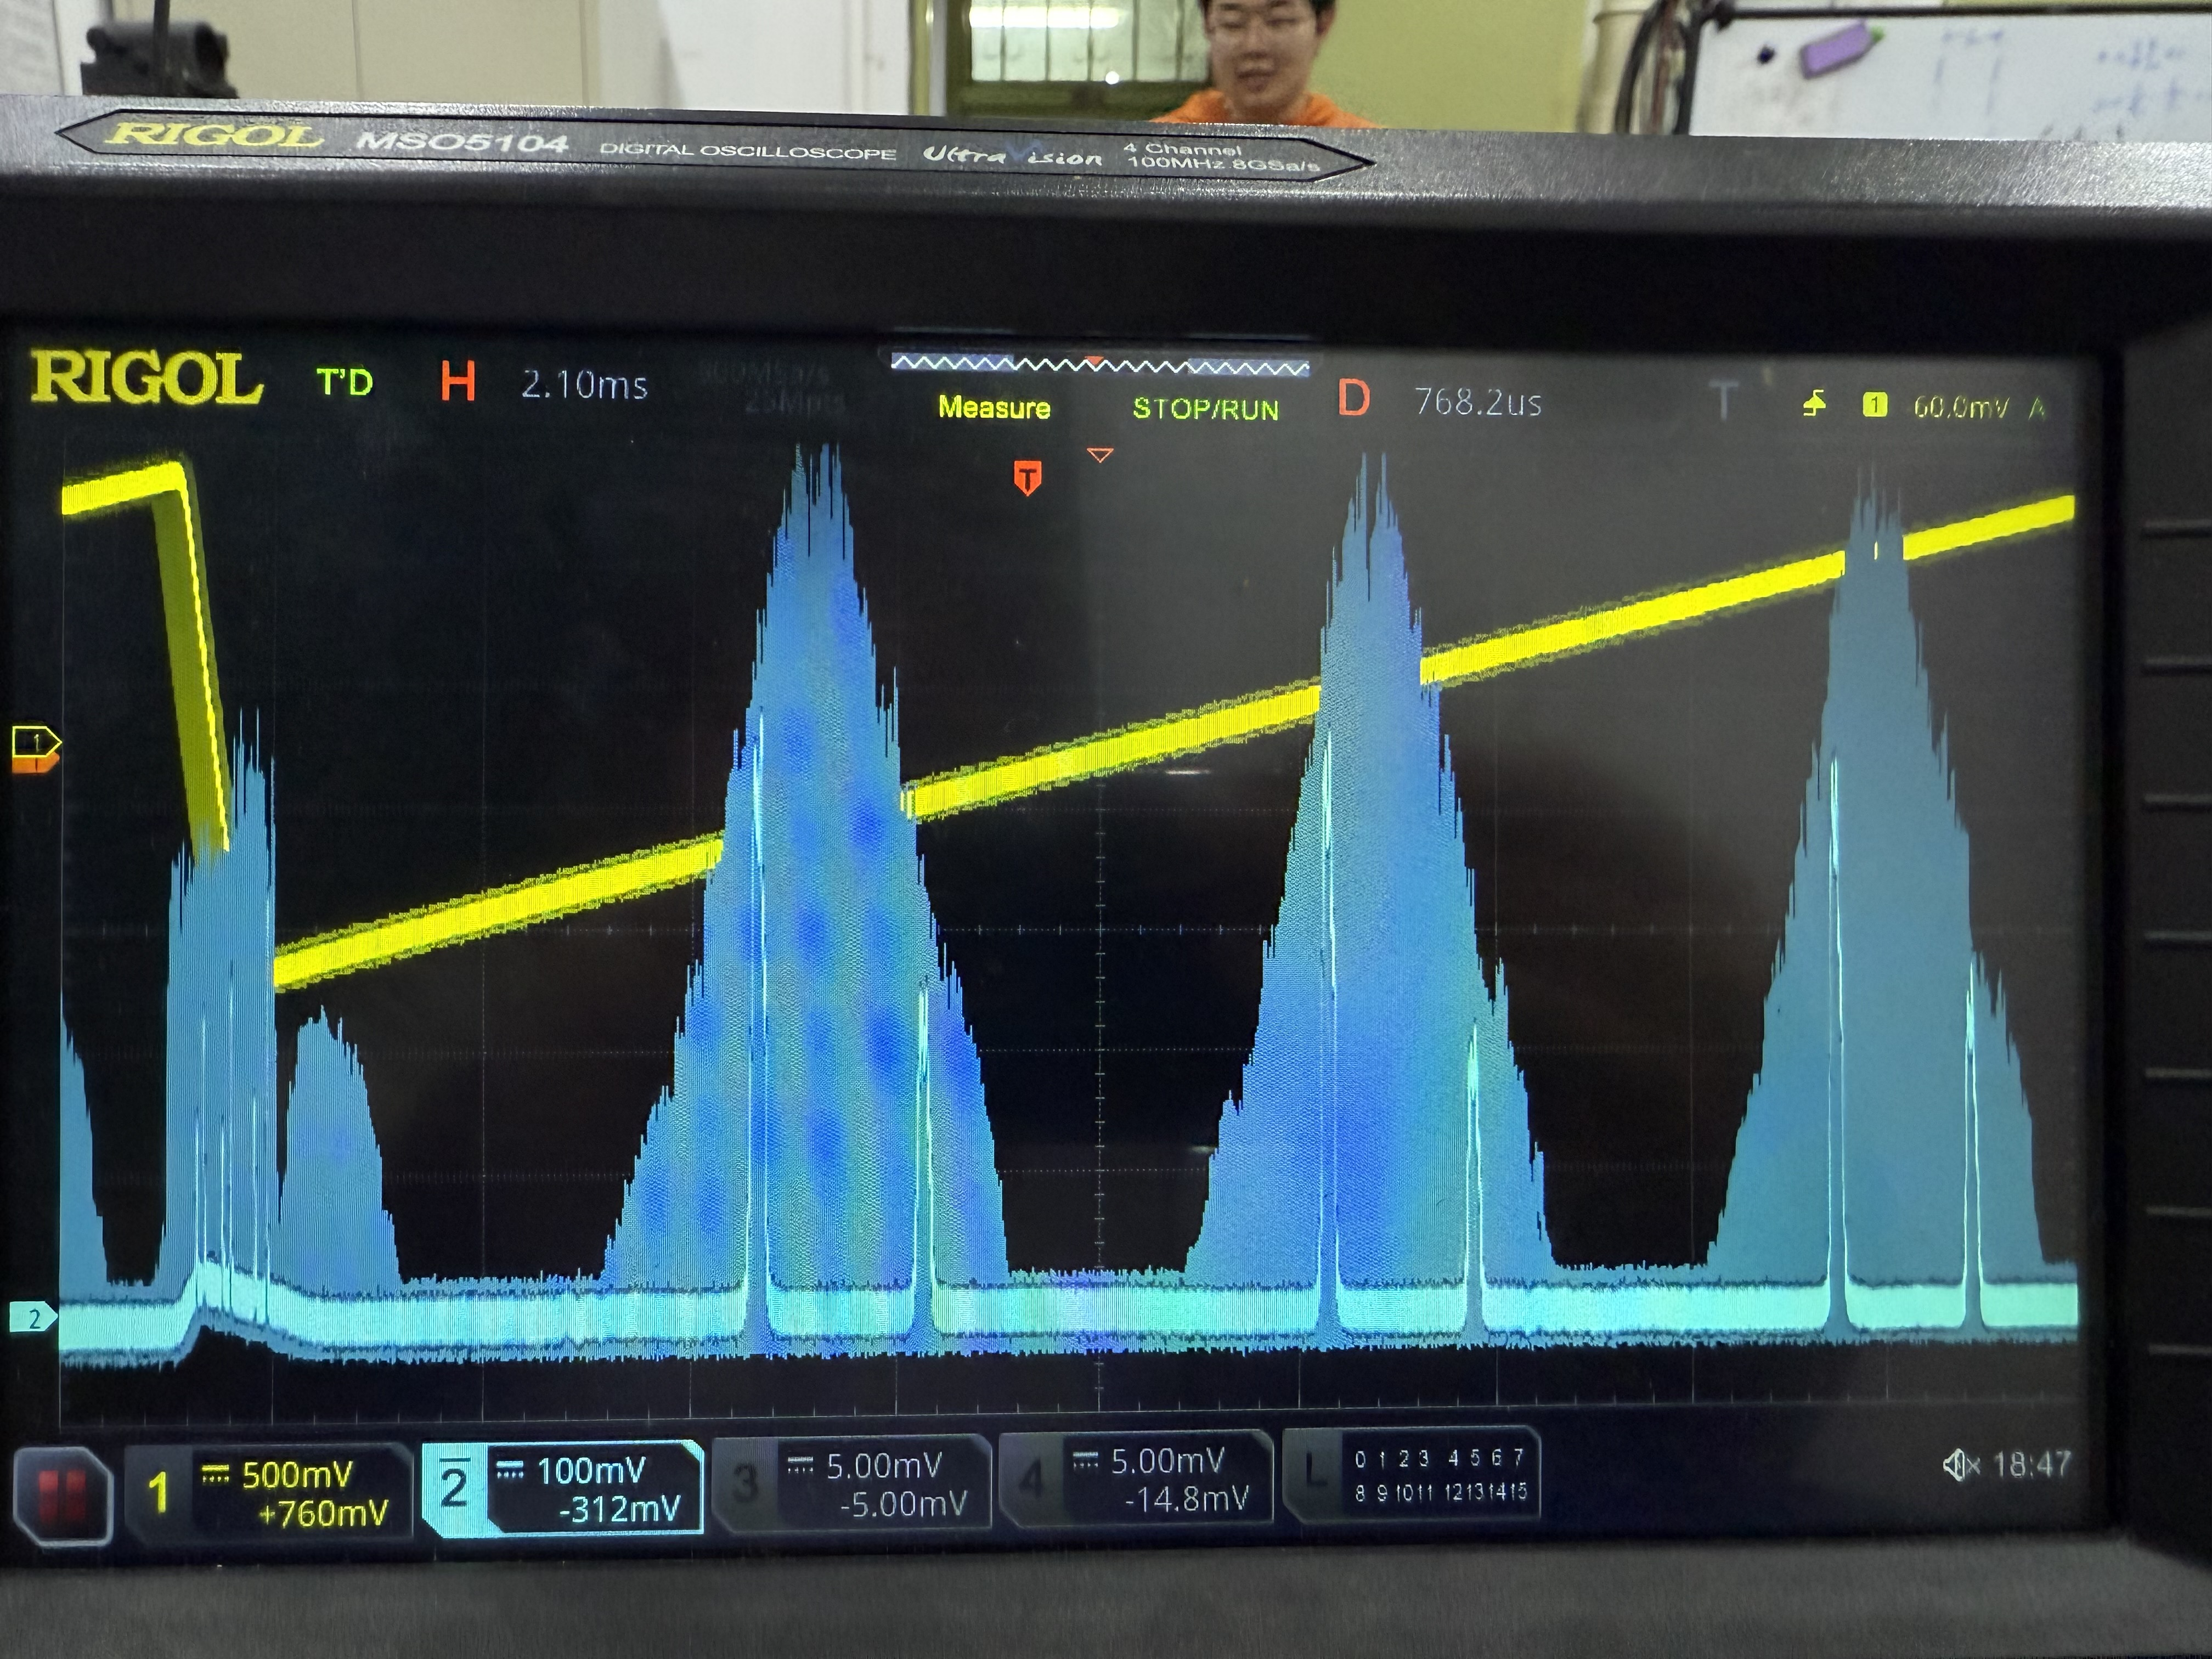
\includegraphics[width=\textwidth,height=4cm]{fig//band} 
        \caption{出光带宽的示波器示例}
        \label{fig:band}
    \end{subfigure}
    \hfill
    \begin{subfigure}{0.47\textwidth}
        \centering
        % 请将图文件 modesplit.png 放置在 fig 目录下
        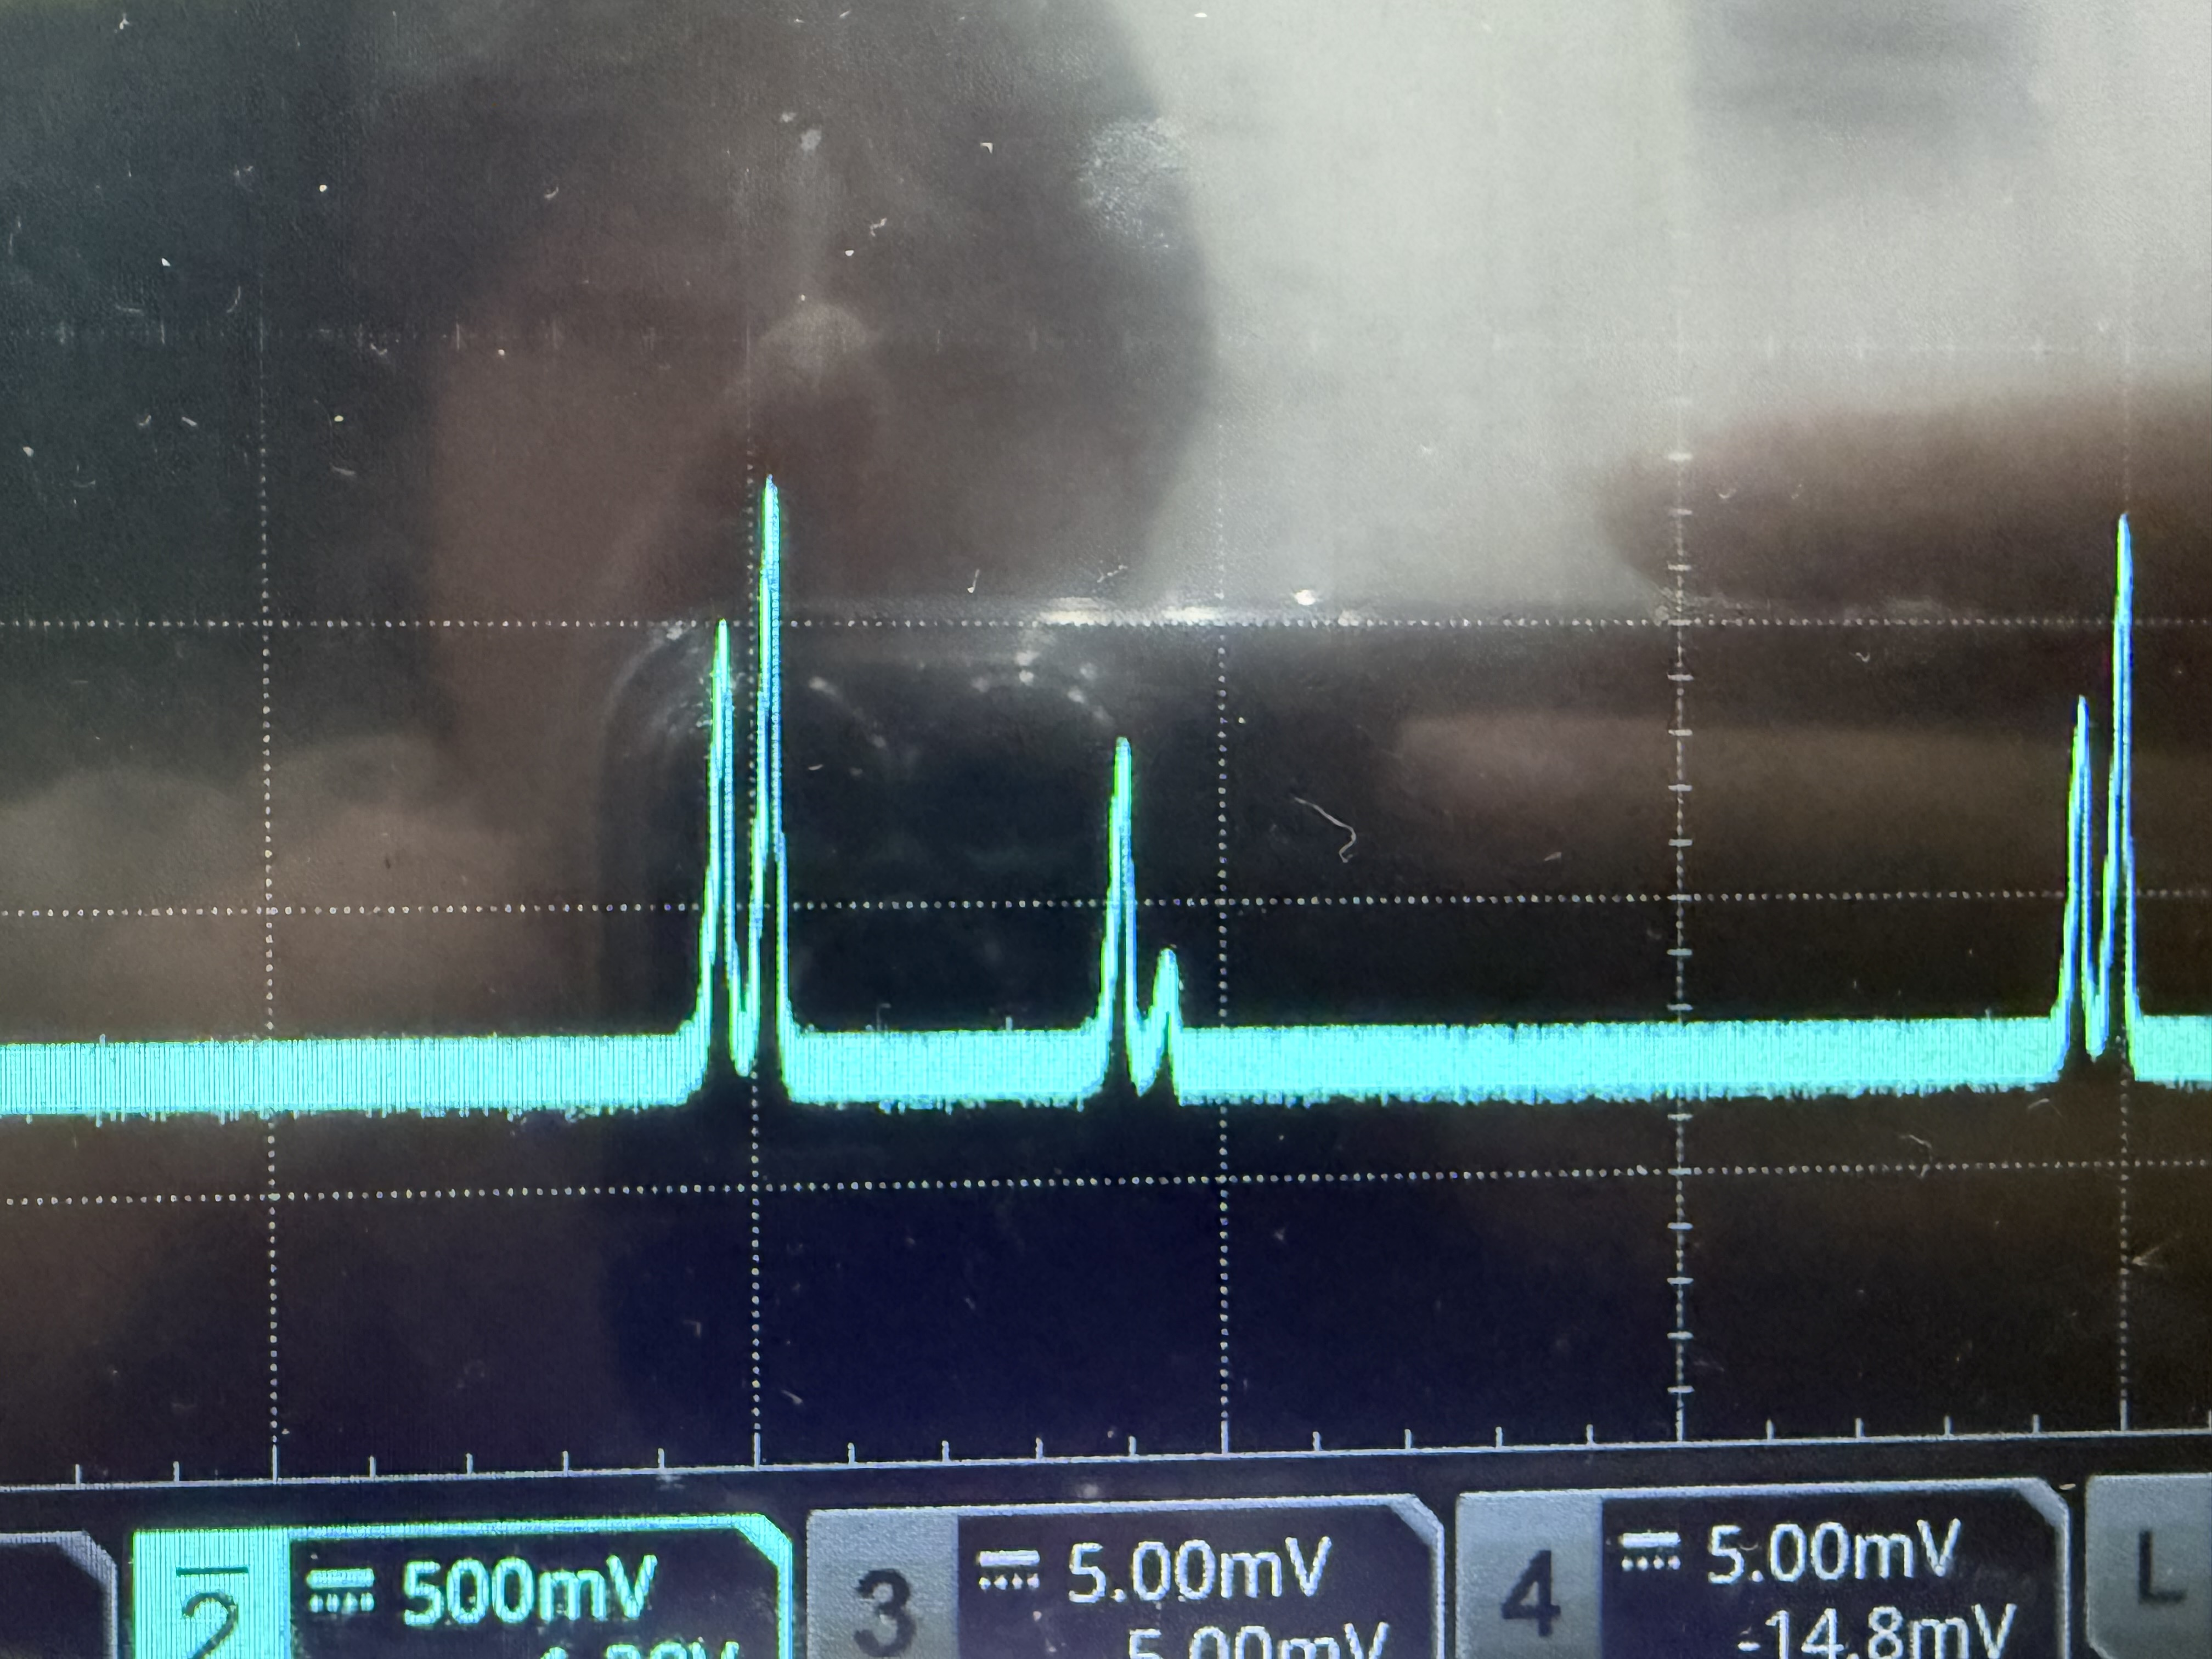
\includegraphics[width=\textwidth,height=4cm]{fig//modesplit}
        \caption{纵模分裂的双峰结构示例}
        \label{fig:split}
    \end{subfigure}
    \caption{氦氖激光器的纵模分裂和模竞争现象观测}
    \label{fig:compete}
\end{figure}

\subsubsection{出光带宽 $\Delta L$ 的测量}

通过改变加在压电陶瓷（PZT）上的电压，激光模式的模谱在示波器上移动。调节示波器至“余辉”模式并将保留时间设为无限长，模谱的移动将在示波器中形成一个带状结构。该带子两端消失点之间的频率间隔，即为激光器工作物质的出光带宽 $\Delta L$。

\begin{table}[h!]
    \centering
    \caption{出光带宽数据记录}
    \label{tab:bandwidth_data}
    \begin{tabular}{|c|c|c|c|c|}
    \hline
    \textbf{参数} & \multicolumn{2}{|c|}{\textbf{数据 1}} & \multicolumn{2}{|c|}{\textbf{数据 2}} \\
    \hline
    $x_{\text{带}}$/ms (端点读数) & -4.368 & -0.168 & 1.659 & 5.544 \\
    \hline
    $\Delta x_{\text{带}}$/ms (计算值) & \multicolumn{2}{|c|}{$(-0.168)-(-4.368)=4.200$} & \multicolumn{2}{|c|}{$5.544-1.659= 3.885$} \\
    \hline
    $\Delta x_{FSR}$/ms (计算值) & \multicolumn{2}{|c|}{$1.659 - (-4.368) = 6.027$} & \multicolumn{2}{|c|}{$5.544- (-0.168) = 5.712$} \\
    \hline
    \end{tabular}
\end{table}

最终得到氦氖激光器的出光带宽：
$$
\Delta L = 1291.39 \mathrm{MHz}
$$

\subsubsection{纵模分裂间距 $\Delta \nu_{\text{split}}$ 的测定}

在激光器内放置石英晶片，通过调整晶轴与光束传播方向的夹角，利用晶片的双折射效应，使每个纵模频率发生分裂，并在扫描干涉仪上观测到双峰结构（图\ref{fig:split}）。

\begin{table}[h!]
    \centering
    \caption{纵模分裂数据记录}
    \label{tab:split_data}
    \begin{tabular}{|c|c|c|c|c|}
    \hline
    \textbf{分裂峰编号} & 1 & 2 & 3 & 4 \\
    \hline
    $x_{\mathbf{I}}$/ms (第一组分裂峰) & -2.638 & -2.444 & -0.9894 & -0.8148 \\
    \hline
    $x_{\mathbf{II}}$/ms (第二组分裂峰) & 3.104 & 3.278 & 4.636 & 4.830 \\
    \hline
    \end{tabular}
\end{table}

\paragraph{纵模分裂间距计算}

通过对两组数据计算，得到自由光谱区的平均时间间隔 $\Delta x_{FSR} = 5.6836 \mathrm{ms}$，纵模分裂间距的平均时间间隔 $\Delta x_{\text{split}} = 0.1842 \mathrm{ms}$。从而计算得到纵模分裂间距为：
$$
\Delta \nu_{\text{split}} = \dfrac{\Delta \nu_{FSR}}{\Delta x_{FSR}}\ \Delta x_{\text{split}} = 60.8 \mathrm{MHz}
$$

\subsubsection{纵模分裂后的偏振关系分析}

为探究纵模分裂的物理本质，实验通过在激光器输出端与扫描干涉仪之间放置偏振片来分析分裂谱线的偏振特性。

\begin{itemize}
    \item \textbf{观测现象：} 当旋转偏振片时，分裂后的两纵模谱线强度此消彼长。即其中一个谱线强度增大时，另一个强度减小直至消失；继续旋转，消失的谱线恢复，另一谱线再次减小直至消失。
    \item \textbf{物理推断：} 偏振片仅允许特定偏振方向的光通过（平行时透射强度最大，正交时透射光消失）。
    \item \textbf{结论：} 这种此消彼长的现象表明，由石英晶体双折射效应产生的两个分裂纵模谱线，其偏振方向是\textbf{相互正交}的。这种模式的频率分裂和偏振正交性是氦氖激光器中著名的纵模竞争现象的体现。
\end{itemize}
    \section{总结}
        本实验成功地通过扫描法 Fabry-Pérot 干涉仪对两根氦氖（He-Ne）激光管的模谱分布进行了测量，并成功观测到激光器的纵模和横模特性。

        同时，在判断长管激光器的横模成分时，仅依靠人眼对光场分布的定性观测存在局限性，难以对复杂的模式叠加做出精确判断。
        
    \begin{thebibliography}{99}
        \bibitem{1}
        北京师范大学物理实验教学中心. 近代物理实验讲义一 (2019)
    \end{thebibliography}

    
\end{document}